\section{Resultados}
\label{sec:resultados}

Os resultados correspondem ao cenário ambiental descrito na seção~\ref{sec:dados}. A leitura parte da rede completa $W$ para distinguir volume e concentração das atribuições e identificar as contrapartes que compõem os perfis setoriais. Em seguida, examina quais relações o filtro destaca e quanto dessa composição permanece representado no backbone $B$.

\subsection{Contas ambientais, volume e concentração}

As duas contas pela ótica da produção $c$ e da demanda $u$ totalizam 683,70 mil Gg de CO\textsubscript{2}, dos quais 392,92 mil Gg estão na diagonal de $F$ e 290,78 mil Gg nas relações entre atividades distintas em $W$. A igualdade entre os totais pela produção e pela demanda decorre da identidade contábil. A parcela intersetorial permite examinar como as mesmas emissões conectam origens e produtos finais, enquanto a diagonal situa o volume atribuído aos produtos finais da própria atividade emissora.

A rede completa tem 67 nós e 4\,290 arestas, com densidade de 97,01\%. Serviços domésticos (9700) é o único nó isolado: sua conta permanece na diagonal de $F$. As outras 66 atividades estão ligadas entre si nas duas direções, com graus iguais a 65. A presença de relações é compatível com a incorporação dos requisitos indiretos em $F$ e pouco distingue os perfis setoriais. O conteúdo desses perfis precisa ser examinado pela distribuição dos pesos.

Entre as 66 atividades conectadas, o número efetivo de contrapartes, $D_2$, varia de 1,58 a 25,04 destinos nas saídas e de 2,13 a 22,10 origens nas entradas; as medianas são 11,50 e 13,93, respectivamente. Embora todas tenham 65 ligações em cada direção, as emissões se concentram de maneira distinta entre as contrapartes. Para compreender sua distribuição entre atividades emissoras e setores de produtos finais, é necessário considerar tanto os volumes atribuídos, medidos pelas forças, quanto sua concentração, expressa por $D_2$. Os painéis A e B da Figura~\ref{fig:indicadores-resultados} permitem examinar essa relação nas atividades com as oito maiores forças de saída ou de entrada em $W$.

Energia (3500) e água, esgoto e resíduos (3680) apresentam as duas maiores forças de saída, com volumes semelhantes: 31,32 e 31,23 mil Gg, respectivamente. Esses volumes, porém, distribuem-se de maneira diferente entre os setores de produtos finais. O número efetivo de destinos é de 20,79 em energia e de 9,88 em água/resíduos, indicando maior concentração das atribuições desta última atividade. Assim, atividades com volumes semelhantes de emissões intersetoriais podem diferir quanto à concentração dessas emissões entre os destinos.

A Tabela~\ref{tab:contas-energia-construcao} relaciona os volumes intersetoriais da Figura~\ref{fig:indicadores-resultados} às contas completas de três atividades. Energia e água/resíduos são mantidas na comparação por apresentarem as duas maiores forças de saída, com volumes semelhantes e concentrações distintas. Construção, com a terceira maior força de entrada, permite examinar a perspectiva do destino e o peso das emissões de outras origens no total atribuído aos seus produtos finais.

\clearpage
\begin{figure}[p]
\centering
\caption{Forças e concentração nas atividades com as oito maiores forças de saída ou de entrada na rede completa, Brasil, 2015.}
\label{fig:indicadores-resultados}
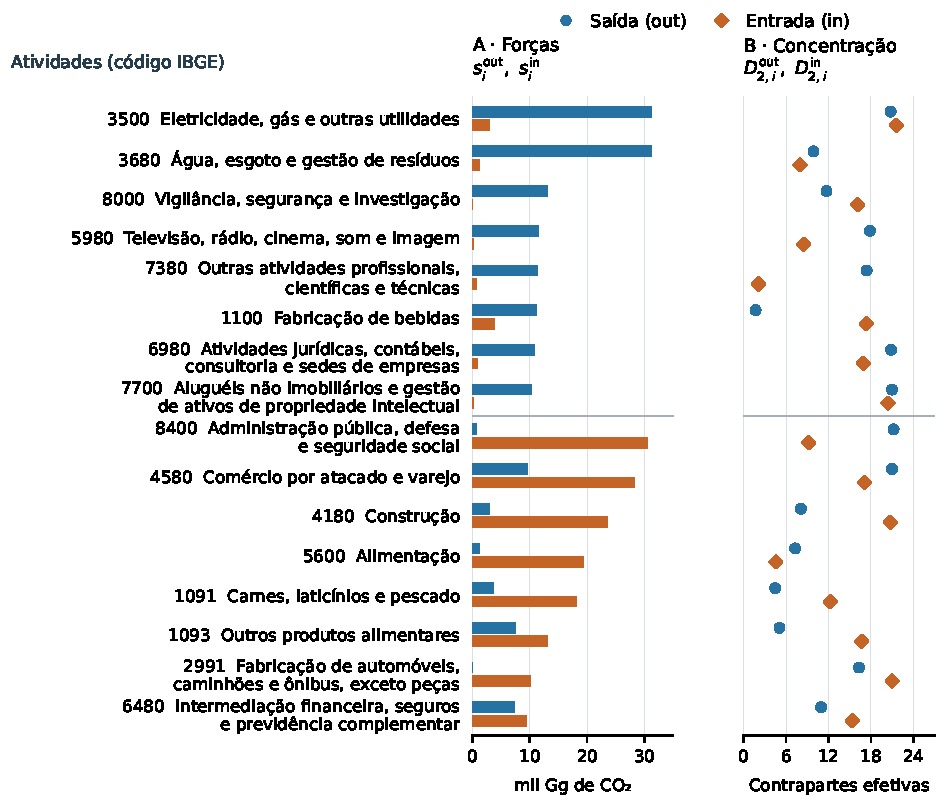
\includegraphics[width=\textwidth,height=0.94\textheight,keepaspectratio]{figuras/indicadores_rede_completa.pdf}
\begin{notas}
Nota: A figura apresenta as 16 atividades que compõem a união das oito maiores forças de saída e das oito maiores forças de entrada da rede completa $W$. Essa rede relaciona as emissões geradas em cada atividade à demanda final dos produtos de outras atividades, considerando apenas atribuições entre atividades distintas. O azul representa a perspectiva de saída, na qual as emissões da atividade indicada são atribuídas aos produtos finais de outras atividades. O laranja representa a perspectiva de entrada, na qual emissões geradas em outras atividades são atribuídas aos produtos finais da atividade indicada.
\par
No painel A, a força de saída, $s_i^{\mathrm{out}}$, mede o volume de emissões próprias atribuído aos produtos finais de outras atividades. A força de entrada, $s_i^{\mathrm{in}}$, mede o volume de emissões de outras atividades atribuído aos produtos finais da atividade indicada. Os volumes são expressos em mil Gg de CO\textsubscript{2}; cada Gg corresponde a mil toneladas.
\par
No painel B, a concentração desses volumes é representada pelo número efetivo de contrapartes, $D_2$, calculado como o inverso do índice de concentração $Y$. O número efetivo expressa quantas contrapartes com participações iguais produziriam a concentração observada. Na saída, as contrapartes são os destinos das atribuições, representados por $D_{2,i}^{\mathrm{out}}$; na entrada, são as origens emissoras, representadas por $D_{2,i}^{\mathrm{in}}$. Quanto menor o número efetivo de contrapartes, maior a concentração das emissões.
\par
Acima da linha horizontal estão as oito atividades com maiores forças de saída; abaixo estão as oito atividades com maiores forças de entrada. Em cada grupo, as atividades aparecem em ordem decrescente da força utilizada na seleção. Os rótulos apresentam os códigos do IBGE e os nomes abreviados das atividades.
\end{notas}
\end{figure}
\clearpage

\begin{table}[!ht]
\centering
\caption{Decomposição das contas de emissões de CO\textsubscript{2} pela produção e pela demanda em energia, água/resíduos e construção, Brasil, 2015 (mil Gg de CO\textsubscript{2}).}
\label{tab:contas-energia-construcao}
\small
\begin{tabular*}{\textwidth}{@{}l@{\extracolsep{\fill}}rrrrrr@{}}
\toprule
\shortstack[l]{Atividade\\(código IBGE)} & \shortstack{Diagonal\\$F_{ii}$} & \shortstack{Saída\\externa\\$s_i^{\mathrm{out}}$} & \shortstack{Entrada\\externa\\$s_i^{\mathrm{in}}$} & \shortstack{Produção\\$c_i$} & \shortstack{Demanda\\$u_i$} & \shortstack{Saldo\\$u_i-c_i$} \\
\midrule
Energia (3500) & 25,30 & 31,32 & 2,92 & 56,62 & 28,23 & $-28,39$ \\
Água/resíduos (3680) & 20,57 & 31,23 & 1,16 & 51,80 & 21,74 & $-30,07$ \\
Construção (4180) & 35,91 & 2,93 & 23,48 & 38,84 & 59,40 & 20,56 \\
\bottomrule
\end{tabular*}
\begin{notas}
Nota: O recorte abrange emissões da produção nacional associadas à demanda doméstica e às exportações, excluindo emissões estrangeiras. Cada linha corresponde à atividade $i$. Produção ($c_i$) contabiliza as emissões na atividade em que ocorrem; demanda ($u_i$) reúne as emissões diretas e indiretas atribuídas aos produtos finais da atividade. A diagonal ($F_{ii}$) corresponde às emissões geradas na própria atividade e atribuídas aos seus produtos finais, incluindo requisitos indiretos. A força de saída, ou saída externa ($s_i^{\mathrm{out}}$), mede as emissões próprias atribuídas aos produtos finais de outras atividades. A força de entrada, ou entrada externa ($s_i^{\mathrm{in}}$), mede as emissões de outras atividades atribuídas aos produtos finais da atividade indicada. Assim, $c_i=F_{ii}+s_i^{\mathrm{out}}$ e $u_i=F_{ii}+s_i^{\mathrm{in}}$; o saldo $u_i-c_i=s_i^{\mathrm{in}}-s_i^{\mathrm{out}}$ é entrada menos saída externa. Diferenças residuais nas somas decorrem do arredondamento.
\par
Seleção: energia e água/resíduos apresentam as duas maiores saídas externas; construção, a terceira maior entrada externa entre as 67 atividades. São casos ilustrativos. Nomes completos: energia elétrica, gás natural e outras utilidades (3500); água, esgoto e gestão de resíduos (3680).
\par
Dados: Matriz de Insumo-Produto do IBGE de 2015 e coeficientes de emissão interpolados de \textcite{sanguinetAzzoni2024}.
\end{notas}
\end{table}

Em energia e água/resíduos, as emissões próprias atribuídas a outros produtos finais superam as emissões de outras origens atribuídas aos seus produtos finais. Por isso, suas contas pela demanda são menores que as contas pela produção; na construção, ocorre o inverso. A diagonal, comum às duas contas, permite situar o peso dessas relações intersetoriais. Na construção, 35,91 mil Gg são gerados na própria atividade e atribuídos aos seus produtos finais, equivalentes a 92,5\% da conta pela produção. Portanto, a pequena saída externa não implica um pequeno volume de emissões próprias. Já na conta pela demanda da construção, as emissões de outras atividades representam 39,5\% do total, enquanto os 60,5\% restantes correspondem à diagonal.

A distribuição das emissões entre origens e produtos finais combina, portanto, atribuições dentro da própria atividade e relações entre atividades distintas. A tabela distingue o volume dessas parcelas; a composição dos perfis, examinada a seguir, identifica quais origens e destinos participam das relações intersetoriais.





\subsection{Composição dos perfis de atribuição}
\label{sec:composicao-perfis}

O contraste de concentração entre energia e água/resíduos na Figura~\ref{fig:indicadores-resultados} envolve participações distintas de destinos compartilhados. Comércio, administração pública e construção aparecem entre os cinco maiores destinos de ambas as atividades (Tabela~\ref{tab:contrapartes-completas}). Entretanto, administração pública reúne 27,22\% das saídas de água/resíduos e 8,16\% das saídas de energia. Essa diferença ajuda a interpretar por que volumes intersetoriais semelhantes se distribuem de forma mais concentrada no primeiro perfil. O peso de administração pública identifica as emissões atribuídas aos produtos finais desse setor, incluindo seus requisitos diretos e indiretos de produção; não corresponde a uma medida das compras diretas do governo junto às atividades emissoras.

\begin{table}[p]
\centering
\caption{Cinco maiores contrapartes nas saídas de energia e de água/resíduos e nas entradas de construção, antes do filtro, Brasil, 2015.}
\label{tab:contrapartes-completas}
\small
\begin{tabular*}{\textwidth}{@{}>{\raggedright\arraybackslash}p{0.57\textwidth}@{\extracolsep{\fill}}rr@{}}
\toprule
Contraparte (código IBGE) & \shortstack{Emissões\\(mil Gg de CO\textsubscript{2})} & \shortstack{Participação no\\volume externo (\%)} \\
\midrule
\multicolumn{3}{@{}l}{\textit{Saídas de energia (3500): destinos dos produtos finais}} \\
Comércio (4580) & 4,224 & 13,49 \\
Administração pública, defesa e seguridade social (8400) & 2,556 & 8,16 \\
Construção (4180) & 2,263 & 7,23 \\
Abate e produtos de carne, laticínio e pesca (1091) & 1,930 & 6,16 \\
Agricultura (0191) & 1,693 & 5,41 \\
Demais 60 destinos & 18,650 & 59,55 \\
Total externo ($s_{3500}^{\mathrm{out}}$) & 31,317 & 100,00 \\
\midrule
\multicolumn{3}{@{}l}{\textit{Saídas de água/resíduos (3680): destinos dos produtos finais}} \\
Administração pública, defesa e seguridade social (8400) & 8,501 & 27,22 \\
Comércio (4580) & 2,964 & 9,49 \\
Saúde privada (8692) & 1,672 & 5,35 \\
Saúde pública (8691) & 1,621 & 5,19 \\
Construção (4180) & 1,592 & 5,10 \\
Demais 60 destinos & 14,880 & 47,65 \\
Total externo ($s_{3680}^{\mathrm{out}}$) & 31,230 & 100,00 \\
\midrule
\multicolumn{3}{@{}l}{\textit{Entradas de construção (4180): origens emissoras}} \\
Produtos de minerais não metálicos (2300) & 2,959 & 12,60 \\
Energia elétrica, gás natural e outras utilidades (3500) & 2,263 & 9,64 \\
Água, esgoto e gestão de resíduos (3680) & 1,592 & 6,78 \\
Comércio (4580) & 1,240 & 5,28 \\
Produtos de metal, exceto máquinas e equipamentos (2500) & 1,037 & 4,42 \\
Demais 60 origens & 14,393 & 61,29 \\
Total externo ($s_{4180}^{\mathrm{in}}$) & 23,484 & 100,00 \\
\bottomrule
\end{tabular*}
\begin{notas}
Nota: cada relação atribui emissões da produção nacional a um setor de produtos finais, incluindo requisitos diretos e indiretos para a demanda doméstica e as exportações; emissões estrangeiras são excluídas. Nas saídas, a atividade indicada no título do bloco é a origem emissora $i$, e cada contraparte é um destino $j$: a emissão é $W_{ij}$, e a participação é $100W_{ij}/s_i^{\mathrm{out}}$. Nas entradas, a atividade indicada é o destino $i$, e cada contraparte é uma origem emissora $j$: a emissão é $W_{ji}$, e a participação é $100W_{ji}/s_i^{\mathrm{in}}$. As forças $s_i^{\mathrm{out}}$ e $s_i^{\mathrm{in}}$ são os volumes externos totais de cada direção. A diagonal, que atribui emissões aos produtos finais da própria atividade emissora, é excluída; os percentuais não usam as contas completas pela produção ou pela demanda.
\par
Seleção: energia e água/resíduos são as duas maiores forças de saída; construção é a terceira maior força de entrada entre as 67 atividades. Cada perfil completo tem 65 contrapartes com atribuição positiva. Mostram-se as cinco maiores, em ordem decrescente de emissão, e as demais 60 agregadas, sem filtragem das relações. Energia $\rightarrow$ construção e água/resíduos $\rightarrow$ construção aparecem nas perspectivas da origem e do destino, com o mesmo volume e denominadores distintos; cada relação deve ser contada apenas uma vez nos totais da rede. Nomes abreviados: energia corresponde a energia elétrica, gás natural e outras utilidades; água/resíduos, a água, esgoto e gestão de resíduos. Diferenças residuais nas somas decorrem do arredondamento dos valores calculados no notebook.
\par
Dados: Matriz de Insumo-Produto do IBGE de 2015 e coeficientes de emissão interpolados de \textcite{sanguinetAzzoni2024}.
\end{notas}
\end{table}
\clearpage

A comparação com construção mostra que uma concentração semelhante pode corresponder a papéis distintos na atribuição das emissões. Na Figura~\ref{fig:indicadores-resultados}, as saídas de energia e as entradas de construção têm números efetivos próximos, ambos de aproximadamente 20,8 contrapartes. Energia distribui emissões próprias entre produtos finais de outras atividades; construção reúne emissões geradas em diferentes origens. Na Tabela~\ref{tab:contrapartes-completas}, produtos de minerais não metálicos, energia e produtos de metal estão entre as principais origens da construção, mas as cinco maiores origens, em conjunto, representam apenas 38,71\% das entradas externas. A parcela intersetorial de 39,5\% da conta pela demanda, identificada na seção anterior, envolve, portanto, uma composição que ultrapassa as principais atividades produtoras de materiais e de energia. Mesmo a atividade de produtos de minerais não metálicos, a maior origem externa, representa 12,60\% das entradas externas e aproximadamente 5,0\% da conta completa pela demanda da construção.

Os perfis também permitem reconhecer as duas perspectivas de uma mesma relação. Construção aparece entre os principais destinos de energia e água/resíduos, que, por sua vez, estão entre as principais origens das entradas de construção. Energia $\rightarrow$ construção representa 7,23\% das saídas externas de energia e 9,64\% das entradas externas de construção. O volume atribuído é o mesmo, mas sua participação muda conforme se examina a distribuição das emissões da origem ou a composição recebida pelo destino. Assim, a descrição das relações exige considerar as duas perspectivas: a posição de uma atividade como origem não determina o peso de cada destino, e a composição de um destino não informa, por si só, quanto ele representa para cada origem. Essa distinção orienta a leitura do filtro nas seções seguintes, em que a seleção de uma ligação é avaliada separadamente na origem e no destino.

\subsection{Seleção das relações e limites de cobertura}

As participações examinadas na seção~\ref{sec:composicao-perfis} mostram que uma relação pode ter importâncias distintas para a origem e o destino. O filtro de disparidade considera essas duas perspectivas ao selecionar as relações do backbone, mantendo as contas e os perfis completos como referência. Para interpretar a distribuição das emissões nessa representação selecionada, é necessário verificar quanto do volume permanece e se a cobertura é semelhante entre atividades e direções.

Em $\alpha=0{,}05$, apenas 13,40\% das relações preservam 70,69\% das emissões intersetoriais (Tabela~\ref{tab:sensibilidade-backbone}). Uma parcela relativamente pequena das relações reúne, portanto, grande parte do volume. Essa redução também omite 29,31\% das emissões entre atividades distintas, que continuam presentes na rede completa e nas contas ambientais. O backbone permite examinar relações selecionadas, mas não substitui a composição completa descrita nas seções anteriores.

A cobertura global, entretanto, não descreve igualmente os dois papéis de uma atividade. A Figura~\ref{fig:indicadores-backbone} mantém as atividades da Figura~\ref{fig:indicadores-resultados} e mostra que, em energia, a seleção representa 99,2\% das saídas, mas apenas 42,1\% das entradas. Assim, o backbone permite acompanhar quase todo o volume de emissões próprias atribuído a outros produtos finais, enquanto deixa de representar a maior parte das emissões de outras origens atribuídas aos produtos finais de energia. Uma lista curta de origens selecionadas não basta para caracterizar a concentração desse perfil: o grau conta relações retidas, a cobertura mede seu alcance em volume e o número efetivo descreve a concentração na rede completa.

A matriz da Figura~\ref{fig:matriz-backbone} acrescenta a localização e o volume das relações selecionadas. Suas linhas permitem acompanhar os destinos das emissões de energia e água/resíduos; a coluna de construção reúne as origens retidas na atribuição aos produtos finais desse setor. Essas perspectivas situam no conjunto das atividades as relações examinadas na Tabela~\ref{tab:contrapartes-completas}. As diferenças de tonalidade mostram que a seleção por importância relativa admite relações de volumes absolutos distintos. Por isso, uma célula mais escura indica maior volume atribuído à relação, mas não maior concentração do perfil nem maior importância relativa para suas duas extremidades.

\begin{table}[htbp]
\centering
\caption{Relações e emissões preservadas pelo filtro de disparidade em diferentes limiares, Brasil, 2015.}
\label{tab:sensibilidade-backbone}
\small
\begin{tabular*}{\textwidth}{@{}l@{\extracolsep{\fill}}rrr@{}}
\toprule
Rede ou limiar & \shortstack{Relações\\n (\%)} & \shortstack{Emissões retidas\\(mil Gg de CO\textsubscript{2})} & \shortstack{Cobertura\\(\%)} \\
\midrule
Sem filtro ($W$) & 4\,290 (100,00) & 290,78 & 100,00 \\
$\alpha=0{,}01$ & 338 (7,88) & 166,88 & 57,39 \\
$\alpha=0{,}05$ (referência) & 575 (13,40) & 205,55 & 70,69 \\
$\alpha=0{,}10$ & 755 (17,60) & 224,92 & 77,35 \\
\bottomrule
\end{tabular*}
\begin{notas}
Nota: cada relação atribui emissões geradas em uma atividade brasileira aos produtos finais de outra, incluindo requisitos diretos e indiretos para a demanda doméstica e as exportações. Emissões estrangeiras e atribuições aos produtos finais da própria atividade emissora (diagonal) são excluídas. A rede completa $W$, sem filtro, contém 4\,290 relações e 290,78 mil Gg de CO\textsubscript{2}. Os percentuais de relações usam como denominador as relações de $W$; a cobertura é a porcentagem das emissões intersetoriais de $W$ preservada em cada seleção. Valores são calculados antes do arredondamento; cada Gg corresponde a mil toneladas.
\par
O parâmetro $\alpha$ é o limiar das probabilidades de cauda do modelo nulo do filtro de disparidade: valores maiores tornam a seleção mais permissiva. Pela regra OU, basta a relação ser selecionada na perspectiva da origem ou do destino. Cada filtro é aplicado à mesma rede completa, sem recalcular as participações após a seleção. Os pesos originais das relações preservadas são mantidos, e as contas completas pela produção e pela demanda não mudam. Todos os casos mantêm 67 atividades, uma isolada e um componente de 66 atividades conectadas quando se desconsidera a direção das relações. O limiar de referência não é considerado ótimo.
\par
Dados: Matriz de Insumo-Produto do IBGE de 2015 e coeficientes de emissão interpolados de \textcite{sanguinetAzzoni2024}.
\end{notas}
\end{table}


A sensibilidade ao limiar delimita essa leitura. Na Tabela~\ref{tab:sensibilidade-backbone}, aumentar $\alpha$ amplia as relações e o volume representados, mas as coberturas agregadas não demonstram estabilidade de cada contraparte ou posição setorial. Mesmo com um componente de 66 atividades nos três limiares, a quantidade de relações e os postos por grau mudam, conforme os diagnósticos do \ref{anexo:diagnosticos}. Mantém-se $\alpha=0{,}05$ como referência convencional. A leitura do backbone precisa, portanto, combinar os volumes completos, a cobertura de cada perfil e a perspectiva responsável pela seleção, examinada a seguir.

\clearpage
\begin{figure}[p]
\centering
\caption{Graus e coberturas do backbone nas atividades com as oito maiores forças de saída ou de entrada na rede completa, Brasil, 2015.}
\label{fig:indicadores-backbone}
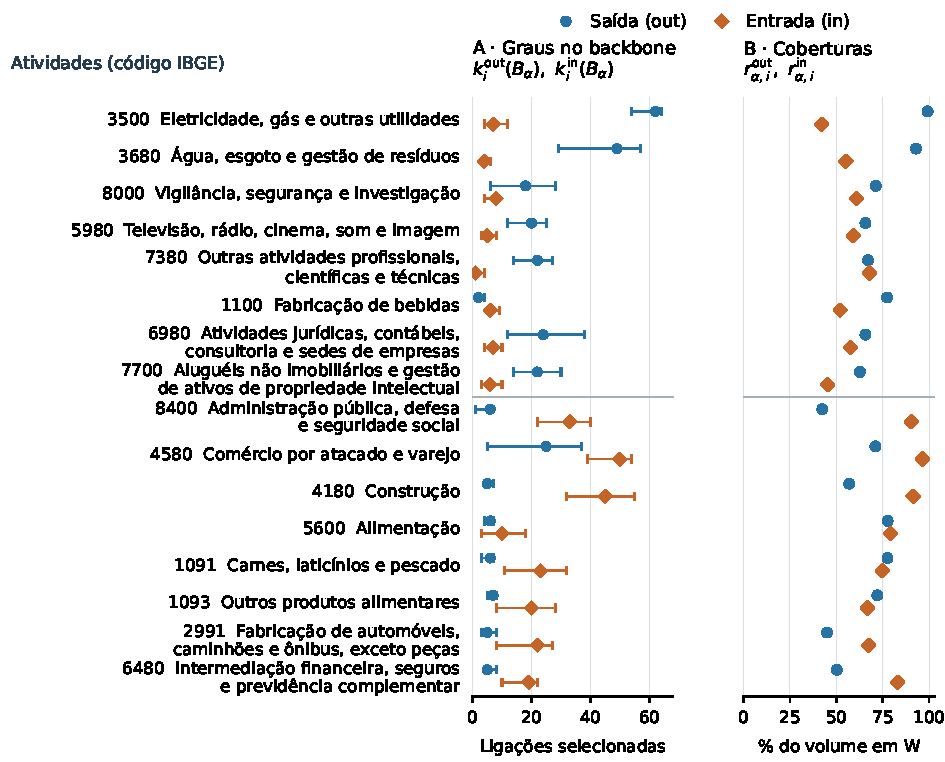
\includegraphics[width=\textwidth,height=0.94\textheight,keepaspectratio]{figuras/indicadores_backbone.pdf}
\begin{notas}
Nota: A figura apresenta os graus e as coberturas do backbone para as 16 atividades que compõem a união das oito maiores forças de saída e das oito maiores forças de entrada da rede completa $W$. A seleção das atividades é feita pelas forças em $W$, antes da filtragem. O backbone $B_\alpha$ é obtido pelo filtro de disparidade, que seleciona ligações com participações excepcionalmente altas na força da origem ou do destino em comparação com uma distribuição aleatória de referência. Os pesos originais das ligações selecionadas são preservados.
\par
O azul representa as ligações de saída da atividade indicada para outros setores de produtos finais. O laranja representa as ligações de entrada, pelas quais emissões de outras atividades são atribuídas aos produtos finais da atividade indicada.
\par
No painel A, os graus de saída e de entrada, $k_i^{\mathrm{out}}(B_\alpha)$ e $k_i^{\mathrm{in}}(B_\alpha)$, indicam o número de ligações preservadas em cada direção. Os pontos mostram os graus obtidos com $\alpha=0{,}05$. As barras horizontais abrangem os graus obtidos entre $\alpha=0{,}01$ e $\alpha=0{,}10$ e mostram a sensibilidade do número de ligações ao limiar do filtro; não são intervalos de confiança.
\par
No painel B, as coberturas de saída e de entrada, $r_{\alpha,i}^{\mathrm{out}}$ e $r_{\alpha,i}^{\mathrm{in}}$, mostram a porcentagem do volume de emissões de cada atividade e direção preservada no backbone para $\alpha=0{,}05$. Cada cobertura compara a soma dos pesos das ligações selecionadas com a força correspondente na rede completa $W$. Assim, o grau informa quantas ligações permanecem, enquanto a cobertura informa quanto do volume original essas ligações representam. Ambos se referem à seleção; o número efetivo de contrapartes da Figura~\ref{fig:indicadores-resultados} caracteriza a concentração dos pesos na rede completa.
\par
Acima da linha horizontal estão as oito atividades com maiores forças de saída em $W$; abaixo estão as oito atividades com maiores forças de entrada em $W$. Em cada grupo, as atividades aparecem em ordem decrescente da força utilizada na seleção. Os rótulos apresentam os códigos do IBGE e os nomes abreviados das atividades.
\end{notas}
\end{figure}
\clearpage
\begin{landscape}
\begin{figure}[p]
\centering
\caption{Emissões de CO\textsubscript{2} nas relações selecionadas pelo filtro de disparidade, $\alpha=0{,}05$, Brasil, 2015.}
\label{fig:matriz-backbone}
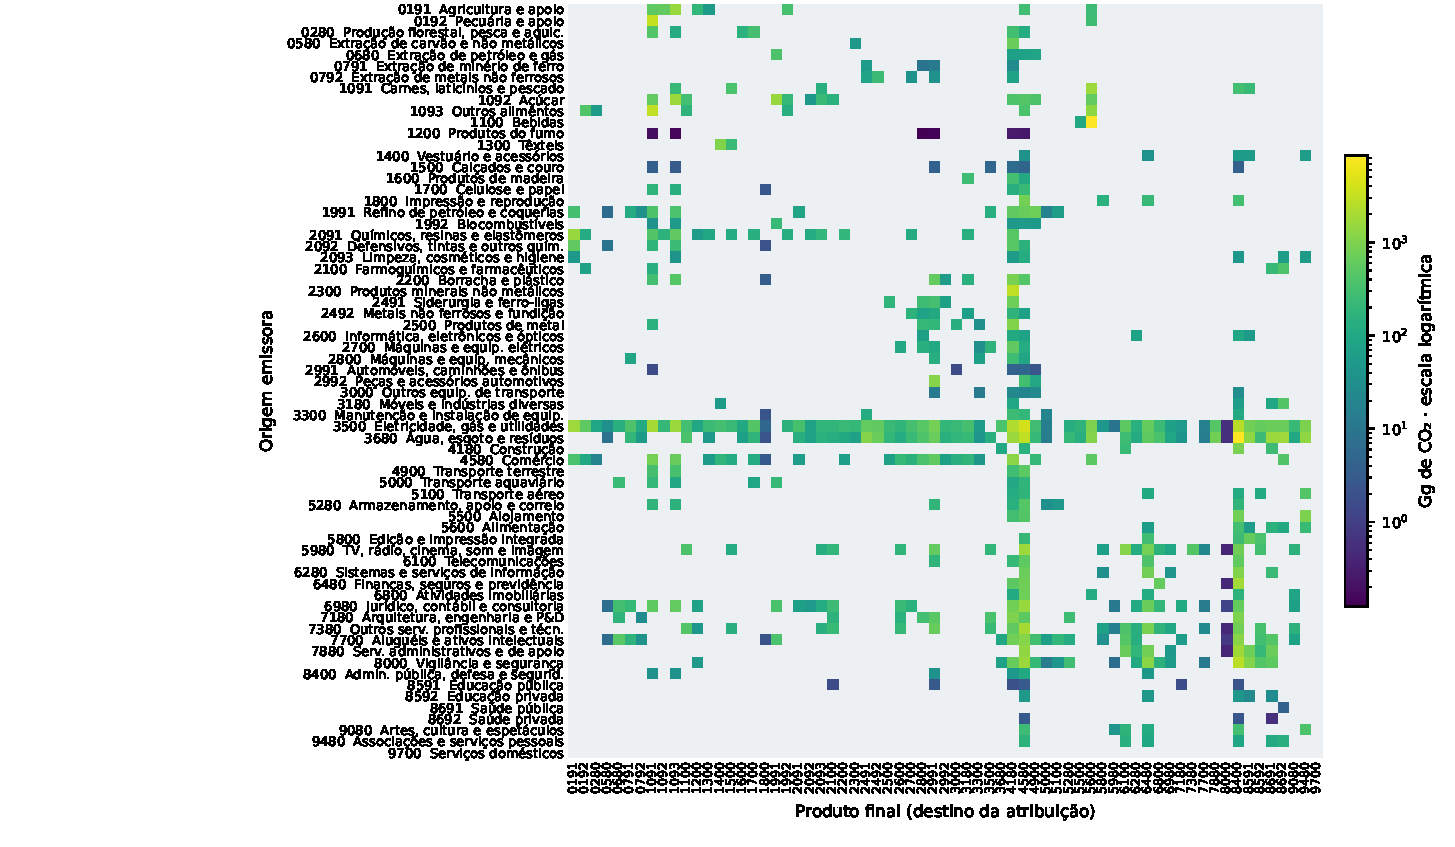
\includegraphics[width=\linewidth,height=0.68\textheight,keepaspectratio]{figuras/matriz_peso.pdf}
\begin{notas}
Nota: cada linha identifica uma atividade emissora e cada coluna, o setor de um produto final. Cada célula colorida representa emissões da origem atribuídas ao destino, incluindo requisitos diretos e indiretos da produção nacional para a demanda doméstica e as exportações; emissões estrangeiras são excluídas. O filtro de disparidade retém a relação se ela é selecionada na perspectiva da origem ou do destino, preservando seu peso original na rede completa $W$. São representadas 575 relações, correspondentes a 70,69\% das emissões intersetoriais de $W$.
\par
A cor mede o volume atribuído à relação, em Gg de CO\textsubscript{2} (mil toneladas): azul claro indica menores volumes e azul escuro, maiores volumes. A escala é logarítmica; intervalos iguais entre as marcas da barra correspondem a multiplicações por dez. As cores não são normalizadas por linha ou coluna e não medem intensidade emissora ou concentração setorial. Cinza indica ausência no backbone, o que não implica necessariamente atribuição nula em $W$. A diagonal é excluída.
\par
Todas as 67 atividades permanecem nos eixos, na ordem do IBGE, com nomes abreviados nas linhas e códigos nas colunas. Os rótulos em negrito destacam as origens energia (3500) e água/resíduos (3680) e o destino construção (4180), examinados nas seções anteriores; não representam outra seleção de relações.
\par
Dados: Matriz de Insumo-Produto do IBGE de 2015 e coeficientes de emissão interpolados de \textcite{sanguinetAzzoni2024}.
\end{notas}
\end{figure}
\end{landscape}

\subsection{Importância local nas duas perspectivas da relação}

A energia aparece como origem destacada na composição das emissões de muitos produtos finais, enquanto a construção constitui um destino destacado para diversas atividades emissoras. Nas saídas de energia, 56 das 62 atribuições retidas são selecionadas apenas pelo teste no destino. Nas entradas de construção, 41 das 45 atribuições retidas são selecionadas apenas pelo teste na origem (Tabela~\ref{tab:motivos-casos}). Esses dois padrões mostram como a importância de uma atividade se manifesta nos perfis de suas contrapartes.

\begin{table}[htbp]
\centering
\caption{Perspectivas de seleção e cobertura das atribuições de CO\textsubscript{2} em energia e construção, $\alpha=0{,}05$, Brasil, 2015.}
\label{tab:motivos-casos}
\small
\begin{tabular*}{\textwidth}{@{}l@{\extracolsep{\fill}}rrrrr@{}}
\toprule
\shortstack[l]{Atividade\\e direção} & \shortstack{Relações\\retidas} & \shortstack{Apenas\\na origem} & \shortstack{Apenas\\no destino} & \shortstack{Na origem\\e no destino} & \shortstack{Cobertura\\(\%)} \\
\midrule
Energia: saídas & 62 & 0 & 56 & 6 & 99,2 \\
Energia: entradas & 7 & 1 & 5 & 1 & 42,1 \\
Construção: entradas & 45 & 41 & 0 & 4 & 91,4 \\
Construção: saídas & 5 & 4 & 1 & 0 & 57,0 \\
\bottomrule
\end{tabular*}
\begin{notas}
Nota: uma relação atribui emissões geradas em uma atividade brasileira (origem) aos produtos finais de outra (destino), incluindo requisitos diretos e indiretos para a demanda doméstica e as exportações. Emissões estrangeiras e atribuições aos produtos finais da própria atividade emissora (diagonal) são excluídas. Saídas distribuem emissões próprias entre outros produtos finais; entradas reúnem emissões de outras origens nos produtos finais da atividade indicada.
\par
O filtro de disparidade compara a participação de cada relação com uma distribuição aleatória de referência para os pesos de cada atividade e direção. Em $\alpha=0{,}05$, a regra OU preserva a relação se ela é selecionada pelo teste na origem ou no destino. As três colunas de motivos identificam a perspectiva responsável pela seleção, independentemente da direção indicada na linha: em entradas de construção, por exemplo, o teste na origem é aplicado às atividades emissoras. As categorias são exclusivas e somam as relações retidas de cada linha. A cobertura é $100$ vezes o volume das relações retidas dividido pelo volume externo completo de saída ($s_i^{\mathrm{out}}$) ou de entrada ($s_i^{\mathrm{in}}$) da atividade $i$ indicada na linha, antes do filtro. Cada linha contabiliza as atribuições do perfil indicado; uma atribuição compartilhada pode aparecer nas linhas de sua origem e de seu destino. Energia corresponde a energia elétrica, gás natural e outras utilidades (3500); construção tem código IBGE 4180. Percentuais são arredondados após o cálculo.
\par
Dados: Matriz de Insumo-Produto do IBGE de 2015 e coeficientes de emissão interpolados de \textcite{sanguinetAzzoni2024}.
\end{notas}
\end{table}

A Figura~\ref{fig:comparacao-perspectivas} compara as participações das emissões de energia atribuídas aos produtos finais de alimentação e de construção e das emissões de produtos de metal atribuídas à construção. Para alimentação, a atribuição representa 3,00\% das saídas externas de energia e 4,86\% das entradas externas do destino. Alimentação ocupa uma posição abaixo dos cinco maiores destinos de energia apresentados na Tabela~\ref{tab:contrapartes-completas}. Ao examinar as entradas de alimentação, o filtro destaca a contribuição de energia à composição das emissões atribuídas aos produtos finais desse setor.

Na atribuição de produtos de metal à construção, o destaque ocorre na perspectiva da origem. Produtos de metal responde por 4,42\% das entradas externas de construção e ocupa a quinta posição entre suas origens na Tabela~\ref{tab:contrapartes-completas}. Para produtos de metal, porém, a construção representa 32,57\% das saídas externas. A construção concentra, portanto, quase um terço das emissões que essa atividade atribui a outros produtos finais. A leitura pela origem identifica essa concentração em um destino específico.

Energia e construção também estão associadas por uma atribuição selecionada pelos dois testes. As emissões de energia atribuídas aos produtos finais de construção totalizam aproximadamente 2\,263 Gg, equivalentes a 7,23\% das saídas externas da origem e a 9,64\% das entradas externas do destino. Nesse caso, energia se destaca na composição recebida por construção, e construção se destaca na distribuição das emissões de energia. As quatro primeiras origens externas da construção na Tabela~\ref{tab:contrapartes-completas} --- produtos de minerais não metálicos, energia, água/resíduos e comércio --- apresentam esse destaque nas duas perspectivas.

\begin{figure}[htbp]
\centering
\caption{Emissões de CO\textsubscript{2} de energia atribuídas à alimentação e à construção e de produtos de metal atribuídas à construção: participações nos volumes externos das origens e dos destinos, Brasil, 2015.}
\label{fig:comparacao-perspectivas}
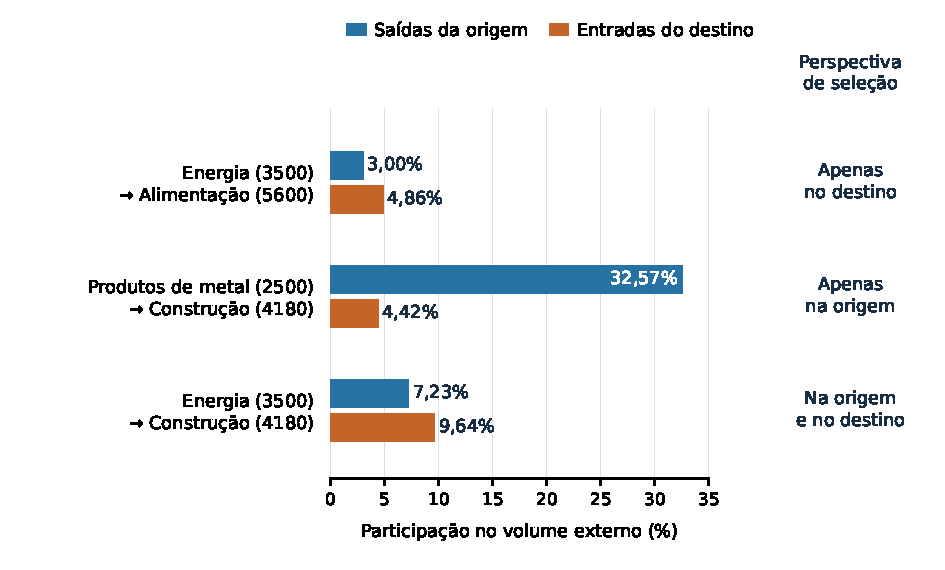
\includegraphics[width=\textwidth,keepaspectratio]{figuras/comparacao_perspectivas.pdf}
\begin{notas}
Nota: cada par de barras apresenta uma atribuição de emissões da atividade emissora $i$ aos produtos finais da atividade $j$, incluindo requisitos diretos e indiretos da produção nacional para a demanda doméstica e as exportações. A barra azul mostra a parcela das saídas externas da origem associada ao destino, $100W_{ij}/s_i^{\mathrm{out}}$; a barra laranja mostra a contribuição da origem às entradas externas do destino, $100W_{ij}/s_j^{\mathrm{in}}$. As duas medidas utilizam o mesmo volume de emissões, $W_{ij}$, e totais de referência distintos: as saídas completas da origem e as entradas completas do destino. Esses totais excluem a diagonal e abrangem as atribuições anteriores ao filtro. O eixo percentual é linear e comum aos três pares de barras.
\par
A indicação sob o título \enquote{Perspectiva de seleção} identifica o teste pelo qual a atribuição é retida no filtro de disparidade, com $\alpha=0{,}05$. O filtro compara as participações observadas a uma distribuição aleatória de referência para cada atividade e direção. A regra OU preserva a atribuição selecionada em pelo menos uma das perspectivas, usando os valores anteriores ao arredondamento. Os exemplos foram escolhidos para apresentar os três casos: seleção apenas no destino, apenas na origem e nas duas perspectivas. Os nomes abreviados correspondem a energia elétrica, gás natural e outras utilidades (3500) e a produtos de metal, exceto máquinas e equipamentos (2500); alimentação e construção têm códigos IBGE 5600 e 4180.
\par
Dados: Matriz de Insumo-Produto do IBGE de 2015 e coeficientes de emissão interpolados de \textcite{sanguinetAzzoni2024}.
\end{notas}
\end{figure}

A Figura~\ref{fig:rede-focos} situa energia e construção no mesmo conjunto de atribuições selecionadas. O destaque alternado permite acompanhar as saídas de energia entre os produtos finais e as origens das emissões atribuídas à construção. A ligação entre energia e construção aparece em azul na vista da origem e em laranja na vista do destino. A passagem entre as duas vistas mostra como uma mesma atribuição participa da distribuição das emissões de uma atividade e da composição dos produtos finais de outra.

A extensão dessas atribuições pode ser lida junto das coberturas da Tabela~\ref{tab:motivos-casos}. O backbone representa quase todo o volume das saídas de energia e a maior parte das entradas de construção. Nas direções inversas, representa 42,1\% das entradas de energia e 57,0\% das saídas de construção. Os perfis completos de saídas de energia e entradas de construção têm concentrações semelhantes, com cerca de 20,8 contrapartes efetivas em ambos, enquanto o filtro retém 62 e 45 atribuições, respectivamente. As coberturas informam o alcance em volume desses conjuntos selecionados, e os números efetivos caracterizam a concentração dos perfis completos.

O predomínio da seleção pelo destino nas saídas de energia e pela origem nas entradas de construção permanece nos três limiares examinados. Entre $\alpha=0{,}01$ e $0{,}10$, o backbone retém de 54 a 64 saídas de energia, com cobertura de 92,12\% a 99,96\%, e de 32 a 55 entradas de construção, com cobertura de 74,31\% a 97,76\% (Tabela~\ref{tab:sensibilidade-casos}). Os cinco maiores destinos de energia permanecem selecionados. A estabilidade desse padrão refere-se à perspectiva que sustenta a maior parte das atribuições retidas em cada perfil.

A composição dos conjuntos selecionados varia com o limiar. Água/resíduos, uma das cinco maiores origens externas da construção, deixa de ser selecionada em $\alpha=0{,}01$, embora represente 6,78\% das entradas externas do setor. Energia $\rightarrow$ construção permanece selecionada pelos dois testes nos três limiares. As atribuições completas e os saldos contábeis são os mesmos nas três seleções; cada limiar define quais atribuições ficam representadas no backbone. Nessa faixa, a permanência dos padrões de seleção de energia e construção convive com mudanças na presença de atribuições específicas.

\clearpage
\begin{figure}[p]
\centering
\caption{Rede de atribuição de emissões de CO\textsubscript{2}: (a) entradas e saídas de energia (3500), $\alpha=0{,}05$, Brasil, 2015.}
\label{fig:rede-focos}
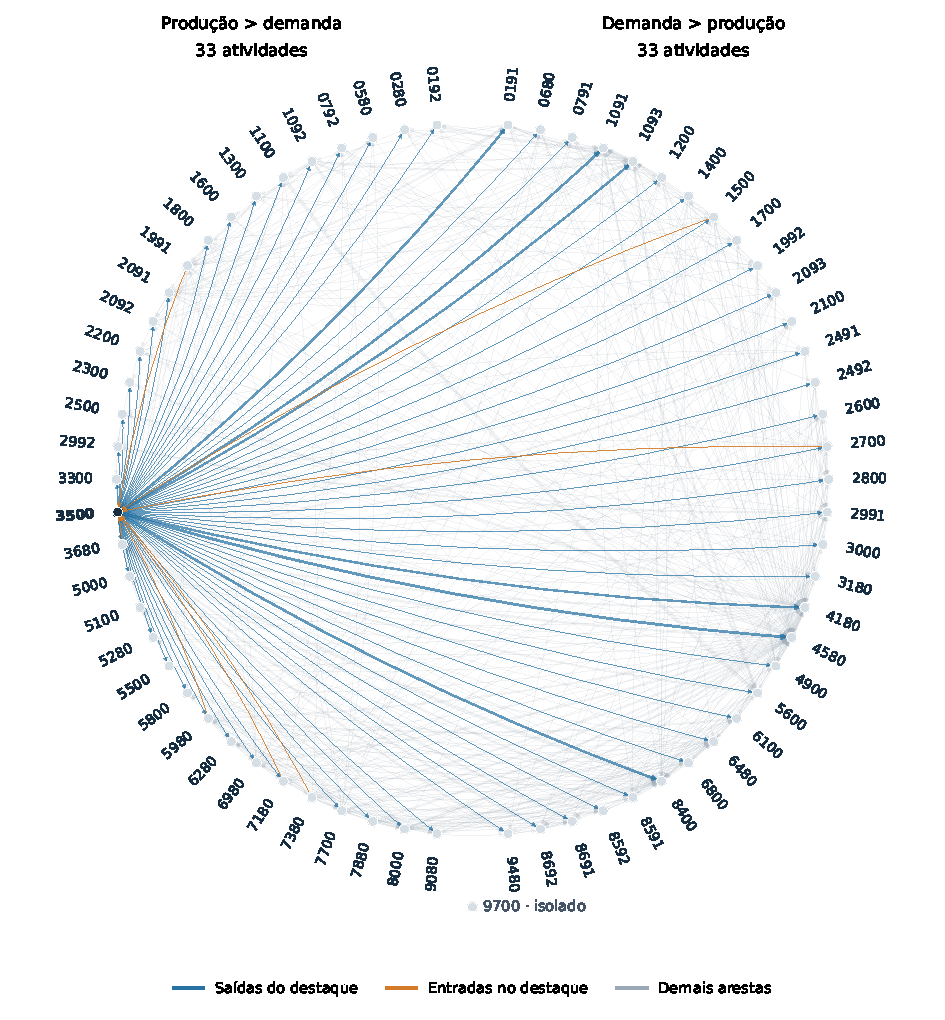
\includegraphics[width=\textwidth,height=0.76\textheight,keepaspectratio]{figuras/rede_foco_3500.pdf}
\begin{notas}
Nota: os 67 nós representam atividades da MIP; cada seta atribui emissões geradas em uma atividade aos produtos finais de outra, incluindo requisitos diretos e indiretos da produção nacional. A figura apresenta as 575 atribuições retidas pelo filtro de disparidade em $\alpha=0{,}05$, equivalentes a 70,69\% das emissões intersetoriais da rede completa, para demanda doméstica e exportações. A diagonal é excluída. Azul destaca as saídas de energia; laranja, suas entradas; cinza, as demais atribuições retidas. Energia tem 62 saídas e sete entradas, que representam 99,2\% e 42,1\% dos respectivos volumes completos.
\par
Os códigos identificam as atividades do IBGE. A área dos nós é uniforme e a espessura das setas cresce com a raiz quadrada do volume de emissões. As posições seguem a ordem do IBGE em dois grupos: à esquerda, 33 atividades cujas emissões pela produção superam as atribuídas pela demanda; à direita, 33 com a relação inversa. Serviços domésticos (9700) é o nó isolado, abaixo dos grupos. Energia corresponde a energia elétrica, gás natural e outras utilidades.
\par
Dados: Matriz de Insumo-Produto do IBGE de 2015 e coeficientes de emissão interpolados de \textcite{sanguinetAzzoni2024}.
\end{notas}
\end{figure}
\clearpage
\begin{figure}[p]
\ContinuedFloat
\centering
\caption{Rede de atribuição de emissões de CO\textsubscript{2}: (b) entradas e saídas de construção (4180), $\alpha=0{,}05$, Brasil, 2015.}
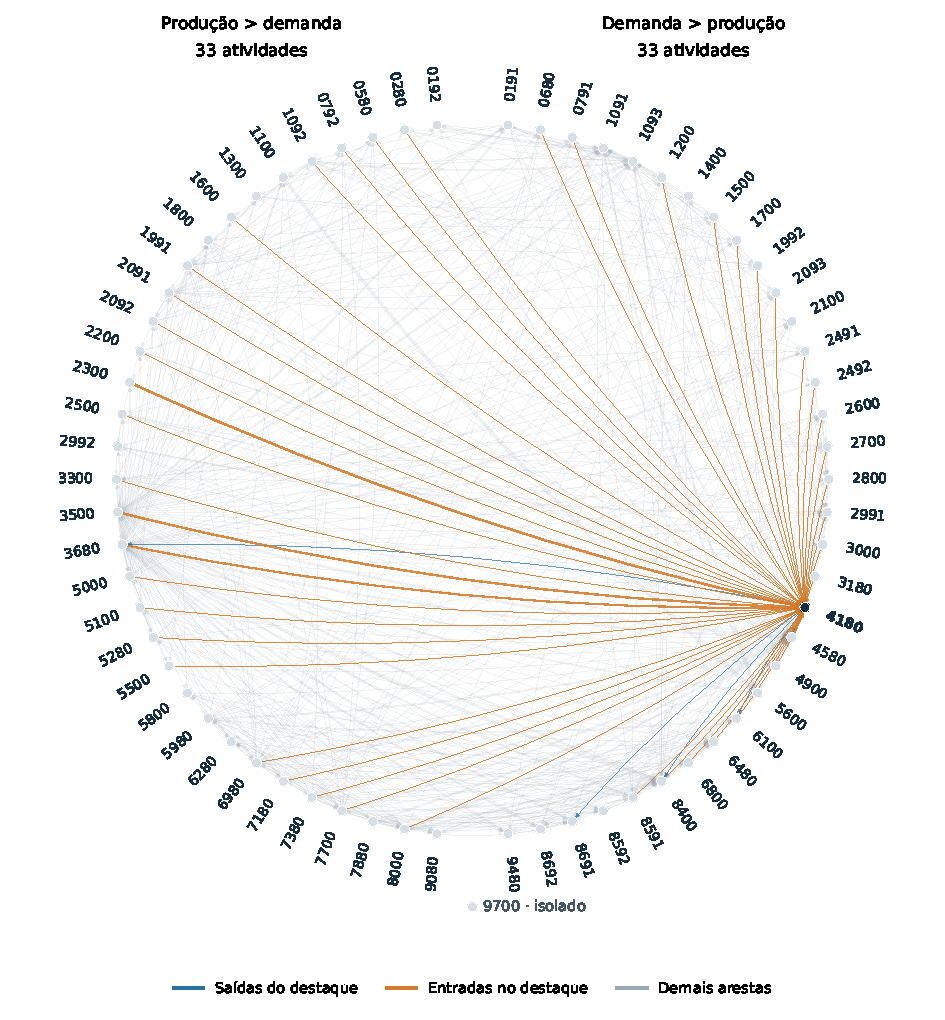
\includegraphics[width=\textwidth,height=0.76\textheight,keepaspectratio]{figuras/rede_foco_4180.pdf}
\begin{notas}
Nota: os 67 nós representam atividades da MIP; cada seta atribui emissões geradas em uma atividade aos produtos finais de outra, incluindo requisitos diretos e indiretos da produção nacional. A figura apresenta as 575 atribuições retidas pelo filtro de disparidade em $\alpha=0{,}05$, equivalentes a 70,69\% das emissões intersetoriais da rede completa, para demanda doméstica e exportações. A diagonal é excluída. Azul destaca as saídas de construção; laranja, suas entradas; cinza, as demais atribuições retidas. Construção tem cinco saídas e 45 entradas, que representam 57,0\% e 91,4\% dos respectivos volumes completos.
\par
Os códigos identificam as atividades do IBGE. A área dos nós é uniforme e a espessura das setas cresce com a raiz quadrada do volume de emissões, na mesma escala da vista de energia. As posições seguem a ordem do IBGE em dois grupos: à esquerda, 33 atividades cujas emissões pela produção superam as atribuídas pela demanda; à direita, 33 com a relação inversa. Serviços domésticos (9700) é o nó isolado, abaixo dos grupos. As posições e as atribuições são as mesmas da vista de energia; o realce identifica os dois sentidos em relação à construção.
\par
Dados: Matriz de Insumo-Produto do IBGE de 2015 e coeficientes de emissão interpolados de \textcite{sanguinetAzzoni2024}.
\end{notas}
\end{figure}
\clearpage
